e^{3}\,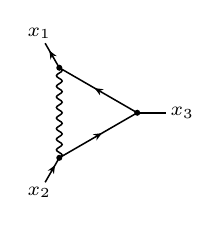
\begin{tikzpicture}[x=0.600cm, y=0.600cm, line width=0.550pt, baseline={([yshift=-0.6ex]0,0)}]
  \draw (1.100,0.000) -- (-0.550,0.953);
  \fill (0.198,0.521) -- (0.314,0.366) -- (0.302,0.461) -- (0.390,0.498) -- cycle;
  \draw (-0.550,-0.953) -- (1.100,0.000);
  \fill (0.352,-0.432) -- (0.160,-0.455) -- (0.248,-0.492) -- (0.236,-0.586) -- cycle;
  \draw plot[smooth, tension=0.7] coordinates {(-0.550,0.953) (-0.507,0.925) (-0.489,0.897) (-0.507,0.869) (-0.550,0.841) (-0.593,0.813) (-0.611,0.785) (-0.593,0.756) (-0.550,0.728) (-0.507,0.700) (-0.489,0.672) (-0.507,0.644) (-0.550,0.616) (-0.593,0.588) (-0.611,0.560) (-0.593,0.532) (-0.550,0.504) (-0.507,0.476) (-0.489,0.448) (-0.507,0.420) (-0.550,0.392) (-0.593,0.364) (-0.611,0.336) (-0.593,0.308) (-0.550,0.280) (-0.507,0.252) (-0.489,0.224) (-0.507,0.196) (-0.550,0.168) (-0.593,0.140) (-0.611,0.112) (-0.593,0.084) (-0.550,0.056) (-0.507,0.028) (-0.489,0.000) (-0.507,-0.028) (-0.550,-0.056) (-0.593,-0.084) (-0.611,-0.112) (-0.593,-0.140) (-0.550,-0.168) (-0.507,-0.196) (-0.489,-0.224) (-0.507,-0.252) (-0.550,-0.280) (-0.593,-0.308) (-0.611,-0.336) (-0.593,-0.364) (-0.550,-0.392) (-0.507,-0.420) (-0.489,-0.448) (-0.507,-0.476) (-0.550,-0.504) (-0.593,-0.532) (-0.611,-0.560) (-0.593,-0.588) (-0.550,-0.616) (-0.507,-0.644) (-0.489,-0.672) (-0.507,-0.700) (-0.550,-0.728) (-0.593,-0.756) (-0.611,-0.785) (-0.593,-0.813) (-0.550,-0.841) (-0.507,-0.869) (-0.489,-0.897) (-0.507,-0.925) (-0.550,-0.953)};
  \draw (-0.550,0.953) -- (-0.850,1.472);
  \fill (-0.759,1.315) -- (-0.736,1.124) -- (-0.699,1.212) -- (-0.605,1.200) -- cycle;
  \draw (-0.550,-0.953) -- (-0.850,-1.472);
  \fill (-0.641,-1.110) -- (-0.795,-1.225) -- (-0.701,-1.213) -- (-0.664,-1.301) -- cycle;
  \draw (1.100,0.000) -- (1.700,0.000);
  \fill (-0.550,0.953) circle (0.064);
  \fill (-0.550,-0.953) circle (0.064);
  \fill (1.100,0.000) circle (0.064);
  \node[font=\scriptsize, inner sep=0pt, anchor=300] at (-0.895,1.550) {$x_{1}$};
  \node[font=\scriptsize, inner sep=0pt, anchor=60] at (-0.895,-1.550) {$x_{2}$};
  \node[font=\scriptsize, inner sep=0pt, anchor=180] at (1.790,0.000) {$x_{3}$};
\end{tikzpicture}